%!TEX root = free234.tex
\chapter{Optimization Problems} %{{{2
In 1st semester calculus you learned how to find the maximal and minimal
values of a function $y=f(x)$ of one variable.  The basic method was as
follows: assuming the independent variable was restricted to some interval
$a\leq x\leq b$, you first look for interior maxima/minima.  These occur at
\emph{critical} or \emph{stationary} points of the function, i.e.\
solutions $x$ of $f'(x)=0$.  You then check the function values at the
endpoints $a$ and $b$ of the interval, to see if they might be maxima or
minima.

To find local maxima and minima you look at the sign of the derivative
$f'(x)$ to see where the function is increasing or decreasing, or you can
apply the \emph{second derivative test.}

This chapter we will see how to solve similar questions about functions of
two or more variables.

First some terminology, and a general fact.


\section{Local and Global extrema}  %{{{2

\label{sec:local-versus-global} 
Let $z=f(x,y)$ be the function whose maximal or minimal values we are
looking for, and let $D$ be the domain of this function.  This domain could
be the largest possible domain for the given function (in case $f$ is
defined by a formula), but it could also be some smaller region which we
ourselves have chosen.  The question we are considering is
\begin{center}
  \itshape What are the largest and smallest values that $f(x,y)$ can have\\
  if the point $(x,y)$ belong to the domain $D$?
\end{center}
\subsection{Definition of global extrema}  %{{{2

\label{sec:def-global-extrema}\itshape 
The function $f$ has a \emph{global maximum} or \emph{absolute maximum} at
a point $(a,b)$ in $D$ if $f(x,y)\leq f(a,b)$ for all points $(x,y)$ in
$D$.

\upshape%
Similarly,\itshape\ the function $f$ has a
\emph{global minimum} or \emph{absolute minimum} at a point $(a,b)$ in $D$
if $f(x,y)\geq f(a,b)$ for all points $(x,y)$ in $D$.

\subsection{Definition of local extrema}  %{{{2

\label{sec:def-local-extrema}\itshape 
The function $f$ has a \emph{local maximum} at a point $(a,b)$ in $D$ if
there is a $r>0$ such that $f(x,y)\leq f(a,b)$ for all points $(x,y)$ in
$D$ which also lie in a disc of radius $r$ centered at $(a,b)$.
\upshape

Local minima are defined analogously.

\subsection{Interior extrema}  %{{{2

\label{sec:interior-extrema} 
Recall that a point $(a,b)$ in a domain $D$ is called \emph{interior} if it
is not a boundary point, or, more precisely, if there is some small $r>0$
such that the disc with radius $r$ centered at $(a,b)$ is entirely
contained in $D$.  We will apply this distinction to the local and global
maxima and minima which we find: an \emph{interior local minimum} is a
local minimum which occurs at an interior point of the domain $D$ of the
function.


\section{Continuous functions on closed and bounded sets}  %{{{2
Before we go into the details of how you can actually find the maxima and
minima, it is good to know the following general fact. It tells us where to
expect maxima and minima.

Let $z=f(x_1,\cdots,x_n)$ be a continuous function defined on some
\emph{closed} and \emph{bounded} region $D$ in $\R^n$.  Remember:
``closed'' means that $D$ contains all its boundary points, and ``bounded''
means that all points in $D$ lie within a ball of some radius $R$ ($D$ does
not ``stretch all the way to infinity''.)

We will also assume that $f$ is continuous on $D$.

\subsection{Theorem about Maxima and Minima of Continuous Functions}  %{{{2
\label{thm:03maxmin-exist}%
\itshape%
A continuous function defined on a closed and bounded region $D\subset
\R^n$ has both a maximum and minimum within that region.  \upshape

This is proved in courses like 522 (2nd semester analysis) or 561
(point set topology).  The proof really doesn't belong here in math
234.



\subsection{Examples}  %{{{2

\label{sec:examples-maxmin-existence} 
\begin{figure}[tb]
   \centering
   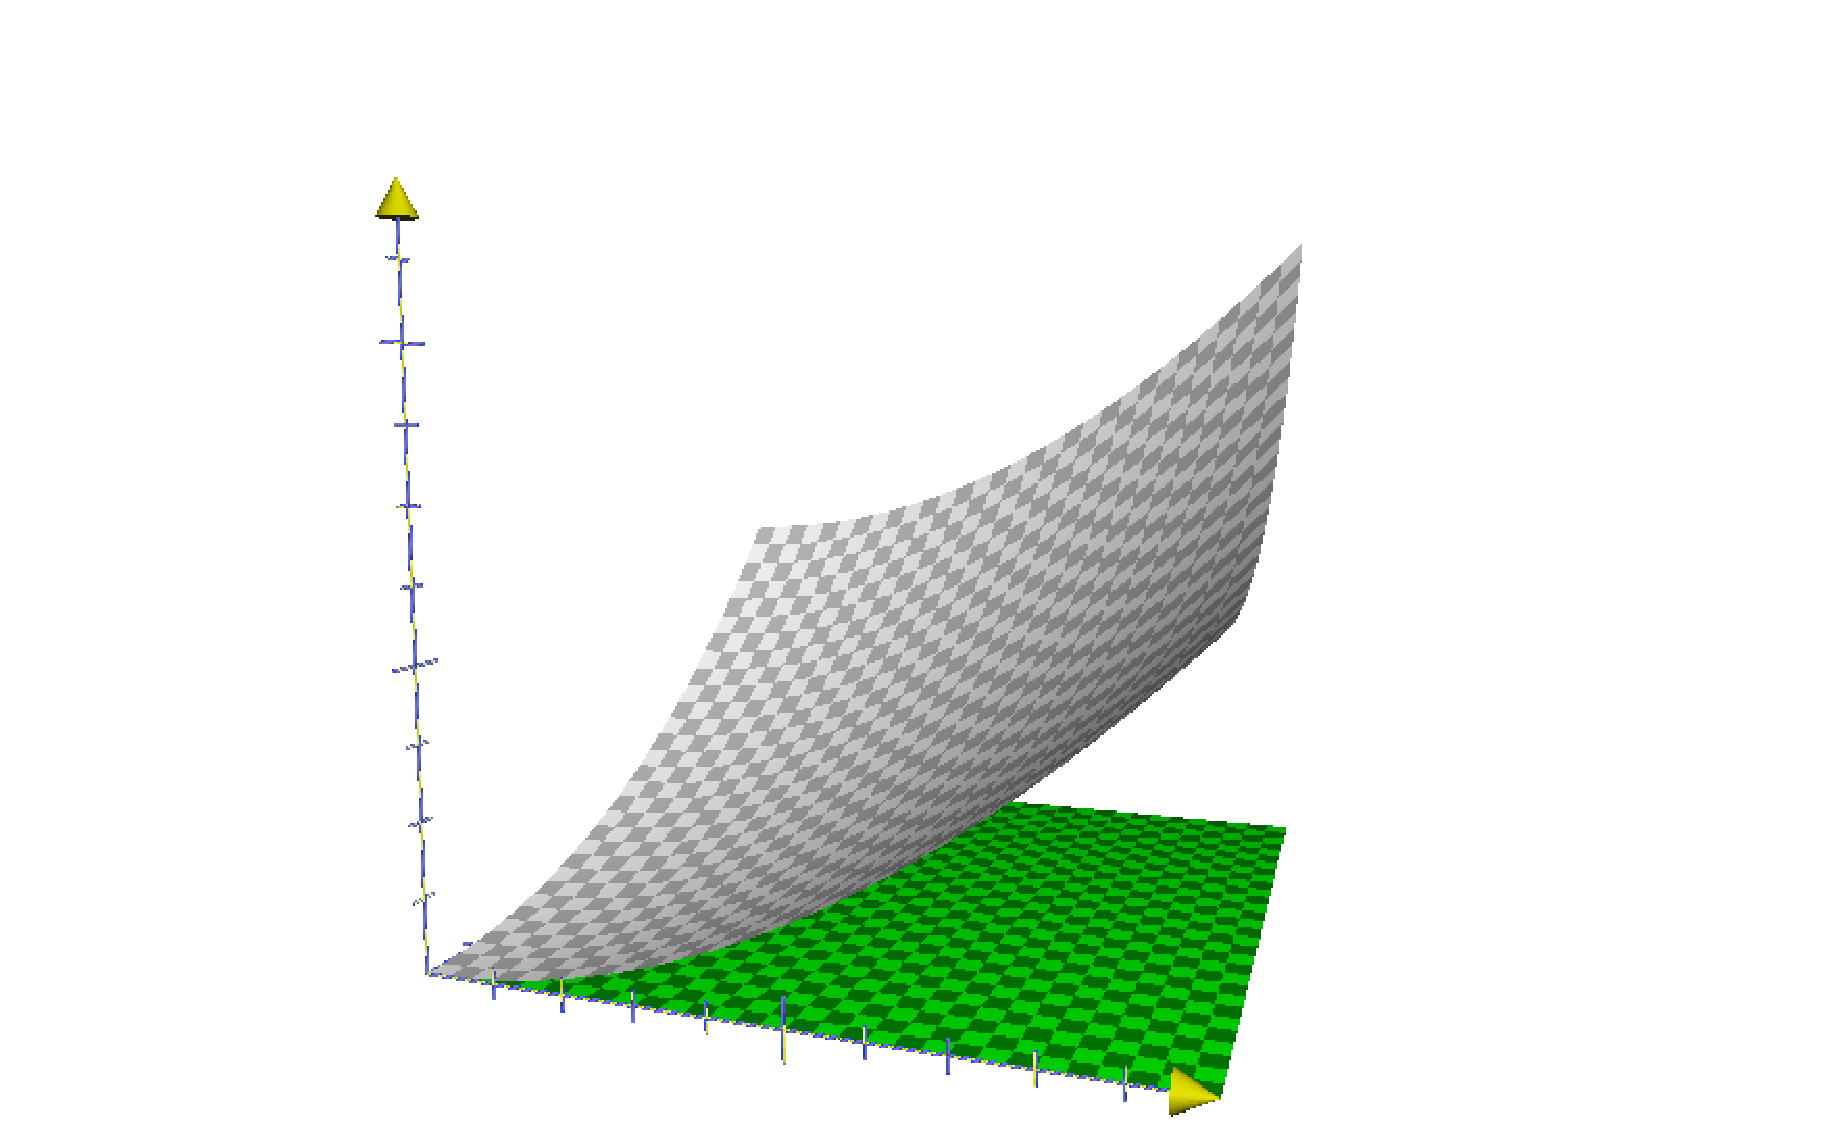
\includegraphics[width=100pt]{figures/03maxmin-on-square.pdf}  
   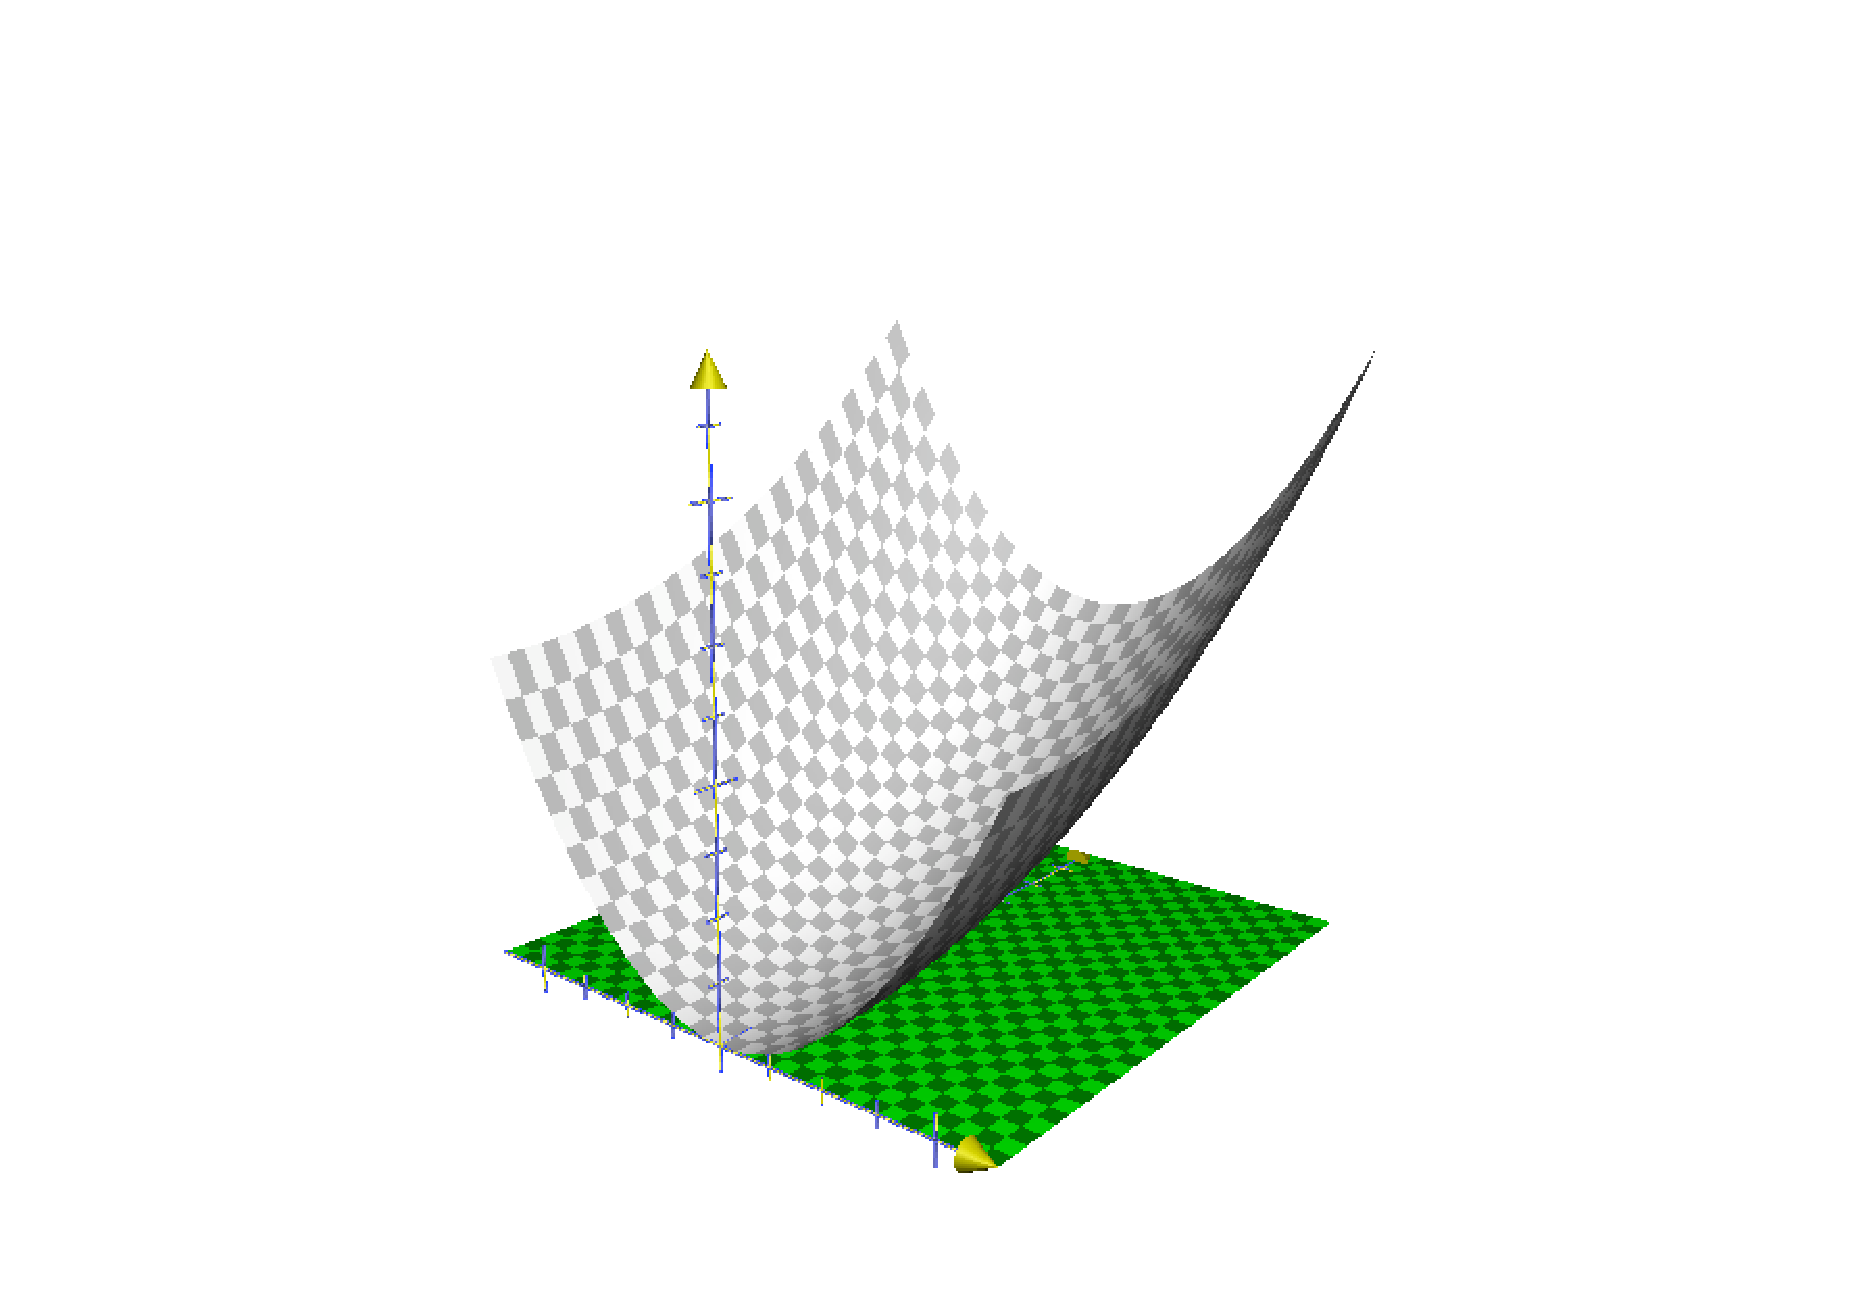
\includegraphics[width=100pt]{figures/03maxmin-on-square2.pdf}  
   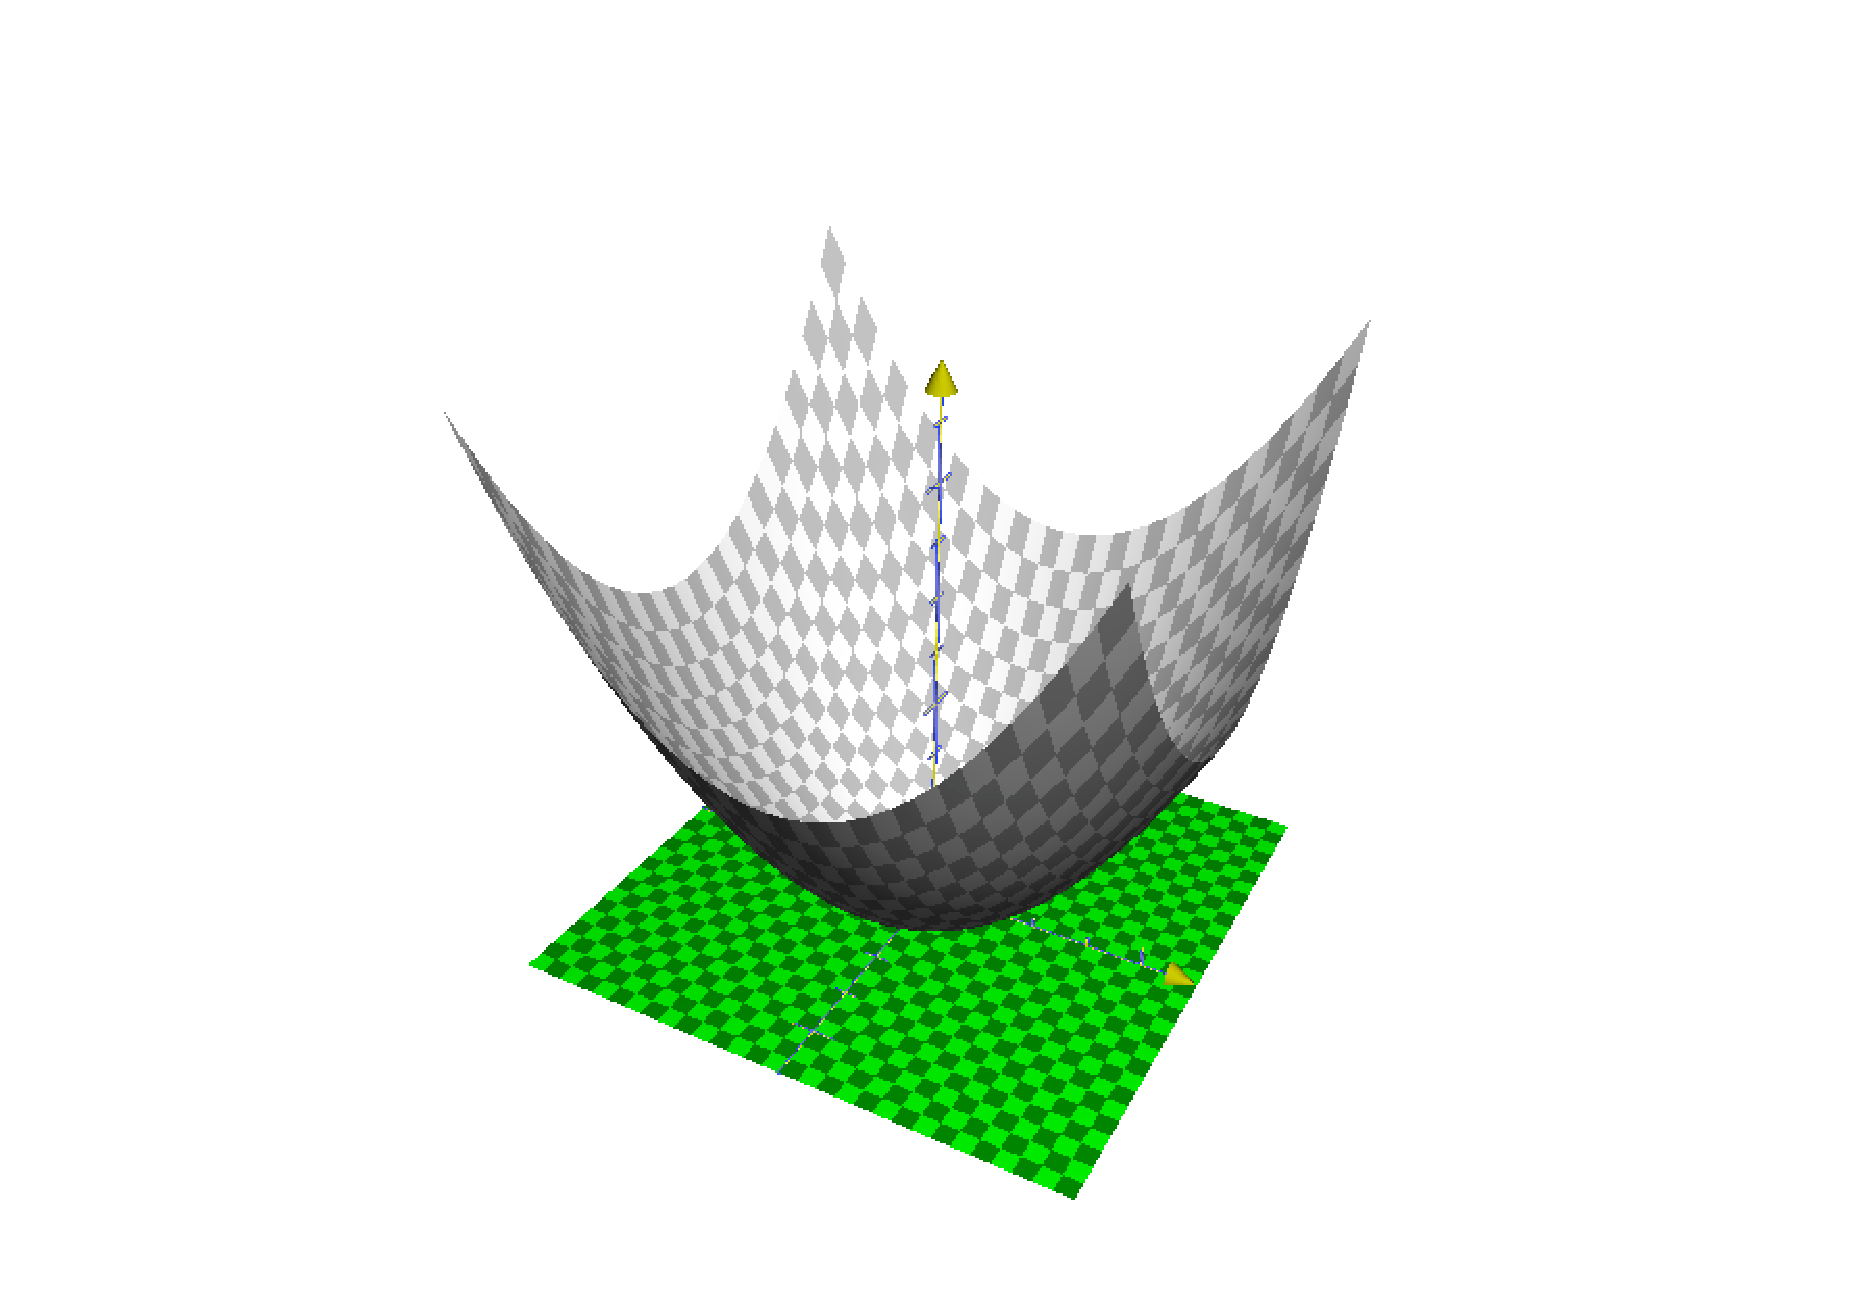
\includegraphics[width=100pt]{figures/03maxmin-on-square3.pdf}
   \caption{The graph of $f(x, y) = x^2+y^2$ from example
     \S~\ref{sec:03maxin-exist-parabolic} on three different rectangles.
     From left to right:\\ (i) $0\leq x\leq1, 0\leq y\leq1$.
     Both max and min are attained at a corner point of the rectangle.\\
     (ii) $0\leq x\leq1, -1\leq y\leq1$, Two maxima, both are attained at
     corner points of the rectangle;
     the minimum is attained at an edge point.\\
     (iii) $-1\leq x\leq1, -1\leq y\leq1$, Four maxima, all attained at
     corner points of the rectangle; the minimum is attained at an interior
     point.}
   \label{fig:03maxin-on-square} 
\end{figure}

\subsubsection{The function $f(x, y) = x^2+y^2$}  %{{{2

\label{sec:03maxin-exist-parabolic} 
This function is continuous, and the square $Q = \{(x, y) : 0\leq x\leq1,
0\leq y\leq1\}$ is bounded, and it contains all boundary points.  Therefore
Theorem~\ref{thm:03maxmin-exist} tells us that $f$ attains both its highest
and lowest values somewhere in the square. The theorem does not say where
these max/min points are.  In this example they are easy to find.  The
function $f(x, y) = x^2+y^2 $ is at its smallest when both $x=0$ and $y=0$,
i.e.\ at the bottom left corner of the square.  And $f(x,y)$ is at its
largest when $x=1$ and $y=1$ both hold.  This happens at the top right
corner of the square.

Note that the boundary of the rectangle $Q$ has two different kinds of
points: it has four corner points, and then all the other points which lie
on the edges.

If you change the rectangle $Q$ then the minimum can appear at a corner
point, a point on an edge, or in an interior point.  See
Figure~\ref{fig:03maxin-on-square}.

For this particular function ($f(x,y) = x^2+y^2$) the maximum can never
appear at an interior point.  This fact is not easy to see right now, but
soon you will be able to prove this using calculus -- it's one of the
exercises.


\subsubsection{A fishy example}  %{{{2

\label{sec:cubic-maxmin-exist} 
Consider the function $f(x, y) = x^2-x^3-y^2$.  Its zero set is the curve
$y^2 = x^2-x^3$, which is shaped like the letter $\alpha$, or like a fish
-- see Figure~\ref{fig:03maxmin-exist-in-fish}.  The function is positive
on the tail ($D_1$) and also on the body ($D_2$) of the fish, it vanishes
on the curve which traces out the fish, and $f$ is negative elsewhere.

Theorem~\ref{thm:03maxmin-exist} does not apply to the region $D_1$ because
$D_1$ is not bounded (it contains the negative $x$-axis).  But the region
$D_2$ is bounded, and our function $f$ is continuous, so
Theorem~\ref{thm:03maxmin-exist} does apply to $D_2$.  The theorem tells us
that the function $f$ has a maximal value and a minimal value in $D_2$.  In
the interior of $D_2$ the function is strictly positive, and on the
boundary of $D_2$ we have $f=0$.  Therefore each boundary point is a
minimum point of $f$ on $D_2$.  The point(s) in $D_2$ where $f$ attains its
highest value must be somewhere in the interior of $D_2$.  In the next
section we will see how to find it (and how to check that in this case
there really only is \emph{one} such point.)

\begin{figure}[ht]
  \centering
  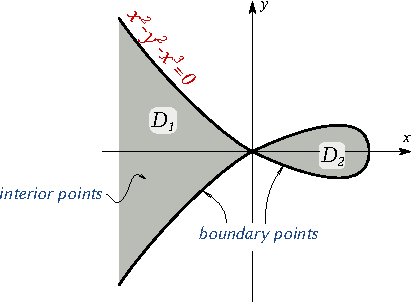
\includegraphics{figures/03maxminexistence.pdf}
  \caption{The region where $f(x, y) = x^2-x^3-y^2$ is positive consists of
    two parts, one bounded (the tear shaped region $D_2$, and the other,
    $D_1$, unbounded.  Theorem~\ref{thm:03maxmin-exist} does not apply to
    the unbounded region, but it does apply to the bounded region $D_2$. In
    that region $f$ must attain its maximum and its minimum.  Since $f=0$
    on the boundary of the region $D_2$, and positive in the interior, $f$
    achieves its lowest value in $D_2$ on the boundary of $D_2$ and its
    highest value somewhere in the interior.
    Theorem~\ref{thm:03maxmin-exist} does not tell you how to find that
    interior point, and allows for the possibility that there might be more
    interior maxima.}
  \label{fig:03maxmin-exist-in-fish} 
\end{figure}



\section{Problems} %{{{2
\problemstyle

\problem Suppose you want to find the \emph{maximize} $f(x, y) =
x^2-x^3-y^2$ over all possible $(x,y)$ with $x\geq 0$ (and no restriction
on $y$ -- this region is called the \textit{right half plane}).

\subprob Explain why you should always choose $y=0$ to maximize this
particular function $f(x, y)$.

\answer If $y\neq0$ then you can increase $x^2-x^3-y^2$ by setting $y=0$.
To put it differently, no matter what you choose for $y$, you always have
\[
f(x, y) = x^2-x^3-y^2 \leq x^2-x^3  =  f(x, 0).
\]
\endanswer

\subprob Use your answer to \textbf{(i)} to find the point $(x, y)$ which
maximizes $f(x,y)$ over the right half plane.

\subprob Does our function $f(x,y)$ have a maximal value if $(x,y)$ can be
any point in the plane?  (hint: what is $f(-1000, 0)$?)

\answer
No, $\lim_{x\to-\infty} f(x, y) = +\infty$, so $f$ has no largest value.
\endanswer

\rmfamily\normalsize

\section{Critical points}  %{{{2
For functions $y=f(x), a\leq x\leq b$, of one variable the standard way of
finding minima (and maxima) is to look for them in two different places:
either the minimum is attained at one of the end points $x=a$ or $x=b$ of
the interval, or else the minimum is attained at an interior point.  At an
interior minimum one has $f'(x) = 0$, so they can be found by solving the
equation $f'(x) = 0$.  The same approach works for functions of two or more
variables.  The basic fact that tells us this is so, is the following
theorem.

\subsection{Local extrema are critical points}  %{{{2

\label{sec:extrema-are-critical} 
\itshape If a function $z=f(x,y)$ defined on a domain $D$ has a local
minimum or local maximum at an interior point $(a,b)$ then one has
\[
\frac{\pd f}{\pd x}(a,b)=0, \text{ and }   \frac{\pd f}{\pd y}(a,b) = 0.
\]
\upshape
\begin{proof}[Picture proof]
  If $f$ has a local maximum at an interior point $(a,b)$ then $f(x, y)
  \leq f(a, b)$ for all $(x,y)$ close to $(a,b)$.  This means that a small
  piece of the graph of $f$ near its local maximum at $(a,b,f(a,b))$ lies
  below the plane $z=f(a,b)$.  This plane must therefore be the tangent
  plane to the graph of $f$.  Being horizontal its slopes are zero, and
  these slopes are exactly the partial derivatives of $f$ at $(a,b)$.  
\end{proof}
\begin{proof}[Frozen variable proof]
  Suppose $f$ has a local maximum at an interior point $(a,b)$ of the
  domain $D$.  Then we can freeze the $y$-variable at the value $y=b$ and
  consider the function of one variable $g(x) = f(x,b)$.  This function has
  a maximum at $x=a$, so by first semester calculus we know that $g'(x) =
  0$.  By definition $g'(x) = f_x(x, b)$, so we conclude that $f_x(a,b) =
  0$.

  By freezing $x$ instead of $y$ you show that $f_y(a,b)=0$ also must hold.

  The same arguments apply to a local minimum.
\end{proof}
\begin{figure}[htb]
  \centering
  
  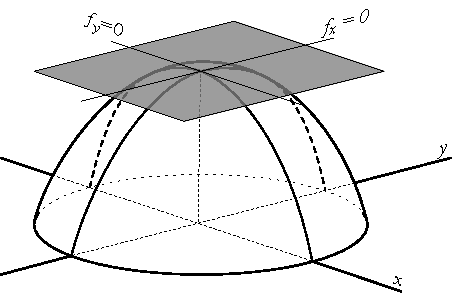
\includegraphics{figures/02localmax.pdf}
  \caption{\emph{Theorem \ref{sec:extrema-are-critical}. } At a local
    maximum the tangent plane to the graph is horizontal.  The partial
    derivatives w.r.t.\ both $x$ and $y$ vanish, and in fact, the
    derivative along \emph{any} path through $(a,b)$ vanishes.  To see a
    picture of a local minimum turn the page upside down.}
\end{figure}

\subsection{Three typical critical points}  %{{{2

\label{sec:criticalpoint-examples} 
Let's find the critical points of the following three functions:
\[
f(x, y) = x^2+y^2,
\quad
g(x, y) = x^2-y^2,
\quad
h(x, y) = -x^2-y^2.
\]
Computing the partial derivatives we find for the first function
\[
\pdd fx = 2x, \quad \pdd fy = 2y.
\]
If $(x,y)$ is a critical point of $f$ then $x$ and $y$ must satisfy the
equations $f_x(x, y) = 0$ and $f_y(x, y) = 0$, in this case, $2x=0$ and
$2y=0$.  So we see that $f$ has exactly one critical point, namely the
origin $(x,y) = (0,0)$.

\textit{Is this critical point perhaps a minimum or a maximum?}  Since
squares can never be negative, $f(x,y) = x^2+y^2$ is always non-negative,
and it is at its smallest when both terms $x^2$ and $y^2$ vanish, i.e.\
$f(x, y)$ has a global minimum at the origin.

Next, let's look at $h(x,y) = -x^2-y^2$.  This function is just $-f(x,y)$,
adn without looking at its derivatives you can tell that it has a global
maximum at the origin.  If you differentiate it you find
\[
\pdd hx = -2x, \quad \pdd hy = -2y
\]
so that the origin is the only critical point of this function too.

The only other function on our list is $g(x, y) = x^2-y^2$.  Its
derivatives are
\[
\pdd gx = 2x, \quad \pdd gy = -2y,
\]
so, once again, the origin is the only critical point.  But, unlike the
previous two functions, $g$ has neither a maximum nor a minimum at the
origin.  You can see this by first looking at what $g$ does on the
$x$-axis, and then what $g$ does on the $y$-axis:

On the $x$-axis you have $g(x, 0) = +x^2$, so $g$ has a \emph{minimum} at
the origin.

On the $y$-axis you have $g(0,y) = -y^2$, so $g$ has a \emph{maximum} at
the origin.

So arbitrarily close to the origin you can find points $(x,y)$ where
$g(x,y)$ is larger than $g(0,0)$, and you can find other points where
$g(x,y)$ is smaller than $g(0,0)$.  Therefore $g$ does not have a local
maximum or a local minimum at the origin.  See
Figure~\ref{fig:most-common-crpts}.

\begin{figure}[htb]
  \centering
  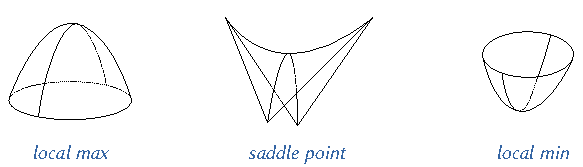
\includegraphics{figures/02threecriticalpoints.pdf}
  \caption{The three most common kinds of critical point.  See
    \S~\ref{sec:criticalpoint-examples}.}
  \label{fig:most-common-crpts} 
\end{figure}

\subsection{Critical points in the fishy example}  %{{{2

\label{sec:critical-fish} 
\textit{What are the critical points of the function $f(x, y) =
  x^2-x^3-y^2$ from \S \ref{sec:cubic-maxmin-exist}?}
We compute the partial derivatives of the function
\[
\pdd fx = 2x-3x^2 = (2-3x)x,\qquad
\pdd fy = -2y.
\]
The equation $f_y=0$ implies that $y=0$, while $f_x=0$ implies $x=0$ or
$x=\frac{2} {3}$.  Therefore $f$ has two critical points: one at the origin
$(0,0)$, and the other at $(\frac23,0)$.

In this example we could have already predicted from the shape of the zero
set of $f$ that $f$ has at least two critical points -- we don't need to
compute the derivatives of $f$ for that.  Namely, the zeroset of $f$ is a
curve which crosses itself at the origin, so the Implicit Function
Theorem~\ref{thm:01implicit-function} (chapter 2) can't hold at the origin,
and hence $f_x=f_y=0$ there.  And in \S~\ref{sec:cubic-maxmin-exist} we
argued that the function $f$ must have a local maximum in the region $D_2$
(Figure~\ref{fig:03maxmin-exist-in-fish}), so $f$ must have at least two
critical points.

\subsection{Another example} %{{{2
\textit{Find the critical points of $f(x,y) =x-x^3-xy^2$. }

\textit{Solution: } The derivatives of our function are
\[
\pdd fx = 1-3x^2-y^2,\qquad
\pdd fy = -2xy.
\]
The critical points are therefore the solutions of the equations
\[
1-3x^2-y^2=0,\qquad -2xy=0.
\]
This is a system of two equation, with two unknowns (that always happens
when you look for critical points, since you're looking for solutions of
$f_x(x,y) = 0$, $f_y(x,y)=0$.)  The second equation, $-2xy=0$, implies that
either $x=0$ or $y=0$ (or both).  We have to treat these two cases
separately:
\begin{quote}
  \begin{trivlist}
  \item [\bf The case $x=0$. ] If $x=0$ then we only have the first
    equation left, which tells us $1-y^2=0$, i.e.\ $y=\pm1$.  We find two
    critical points with $x=0$, namely, $(0,1)$ and $(0,-1)$.
  \item [\bf The other case, $x\neq0$. ] If $x\neq0$, then the second
    equation ($-2xy=0$) implies $y=0$.  Substitute this in the first
    equation and you find $1-3x^2=0$, i.e.\ $x=\pm\frac{1} {3}\sqrt{3}$, so
    that we have two critical points with $x\neq0$, namely,
    $(-\frac13\sqrt3, 0)$ and $(\frac13\sqrt3, 0)$.
  \end{trivlist}
\end{quote}
\parpic{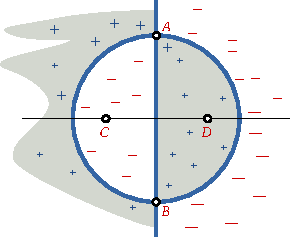
\includegraphics{figures/03example-criticalpoints.pdf}}
The conclusion is that this function has four critical points, two on the
$x$-axis, and two on the $y$-axis.  Without looking into this in any
further detail we don't know if any of these points are local maxima or
minima.  In general the second derivative test (to be explained in
\S~\ref{sec:second-deriv-test}) will provide this information.  For this
example a look at the zero set of $f$ also helps us figure out what kind of
critical points we have found.  Since $f$ factors as $f(x, y) =
x(1-x^2-y^2)$, you see that its zero set consists of the line $x=0$
(a.k.a.\ the $y$-axis), and the unit circle $x^2+y^2=1$.  In the above
picture $f>0$ in the grey region, and $f<0$ in the white area.  Consider
the right half of the unit disc.  The function is non-negative in the
interior, and zero on the boundary of this region.  Just as in the ``fishy
example'' of \S~\ref{sec:cubic-maxmin-exist}, we have another case where
the maximum of the function must be attained at one or more interior points
of the right half of the unit disc.  According to our computation $f$ only
has \textit{one} critical point in the right half circle, and therefore
this point must be a local maximum of the function.  Conclusion:
$D=(\frac13\sqrt3,0)$ is a local maximum.

In the same spirit you can argue that $f$ has a local minimum at $C$.

The other two points $A,B$ are neither local maxima nor minima, since
\textit{arbitrarily close to $A$ or $B$} there are both points $(x,y)$ with
$f(x,y)$ positive, and points with $f(x,y)$ negative.  The points $A$ and
$B$ turn out to be ``saddle points.''

\subsection{One more example: Linear Regression}  %{{{2

\label{sec:linear-regression} 

Suppose you are measuring two quantities $x$ and $y$ in some experiment,
and suppose that you expect that there is a linear relation of the form
$y=ax+b$ between $x$ and $y$.  If you have a set of data points $(x_k,
y_k)$ from some experiment, then what do they tell you about $a$ and $b$?
\emph{Which choice of coefficients $a$ and $b$ bests fits your data? }
Because of experimental errors you would not expect your data points to lie
on a straight line, but instead, you expect them to be clustered around a
straight line.  You could print the data points and draw a straight line by
hand that looks like the best match -- then you measure $a,b$ from your
drawing.  A more systematic approach is to first define what you mean by
``best match'' and then find the line that best matches according to your
chosen criterion.

A very common criterion is the least-mean-square-fit.  Imagine you have $N$
data points, $(x_1,y_1)$, \ldots $(x_N, y_N)$, and you choose the line with
coefficients $a$ and $b$.  Most data points $(x_k, y_k)$ will then probably
not lie on the line $y=ax+b$, and one uses
\[
E_k = \bigl(ax_k+b-y_k\bigr)^2
\]
as a measure for the mismatch between the data point $(x_k, y_k)$ and the
line $y=ax+b$.  Adding all these errors we get the total ``mean square''
error
\[
E= E_1 + \cdots + E_N.
\]
If we think of all the numbers $x_1, \ldots, x_N, y_1, \ldots, y_N$ as
given constants (after all, you measured them, so you shouldn't change them
any more), then the total error only depends on the coefficients $a$ and
$b$.  It is a measure for how well the line $y=ax+b$ fits our data points,
and the common method of \emph{linear regression} consists in choosing the
coefficients $a$ and $b$ so as to minimize this error $E$.

\begin{figure}[htb]
  \centering
  \begin{picture} (300.000000,162.461538)(0,0)
    \put(0.0, 0.0){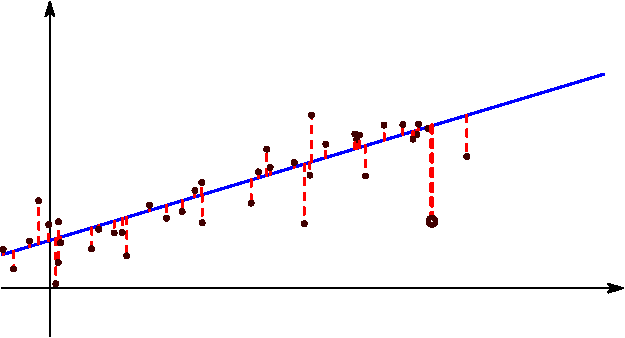
\includegraphics{02linearregression.pdf}}
        \put(241.69, 116.18){\sffamily\itshape \makebox[0pt][l]{\rotatebox{16.699244}{$y=ax+b$}}}
    \put(207.31,  46.02){\sffamily\itshape \makebox[0pt][c]{$(x_k, y_k)$}}
    \put(211.31,  78.94){\sffamily\itshape \makebox[0pt][l]{$\bigl|ax_k+b-y_k\bigr|$}}

\end{picture}

  \caption{Which line best fits a set of data points?}
\label{fig:linear-regression} 
\end{figure}

This leads us to the problem of finding the critical points of the total
error $E$ as a function of $a$ and $b$.  To do this we need to write the
total error in a way that clearly shows how it depends on $a$ and $b$.
First we expend the error $E_k$ associated with the $k^{\rm th}$ data point:
\[
E_k = \bigl(ax_k+b-y_k\bigr)^2
=x_k^2\, a^2 + 2x_k \, ab + b^2 -2x_ky_k\, a - 2 y_k\, b + y_k^2 .
\]
Adding this over all data points, and collecting terms with the same powers
of $a$ and $b$ leads to
\[
E(a,b) = A\,a^2 +2B\, ab + C\, b^2 - 2D\,a -2E\, b +F,
\]
where
\[\textstyle
A = \sum x_k^2,\;\;
B=\sum x_k,\;\;
C=N,\;\;\;
D= \sum x_ky_k,\;\;
E= \sum y_k,\;\;
F= \sum y_k^2
\]
and ``$\sum$'' represents summation over $k=1, 2, 3, \cdots, N$.  The
numbers $A, B, \cdots, F$ are known constants which you compute from
the data points $(x_1,y_1), \cdots, (x_N,y_N)$ that came out of your
experiment.

The domain of the function is the whole plane (all possible
combinations are conceivable), and hence, if there is a ``best'' choice of
$(a,b)$, i.e.\ one which minimizes $E(a,b)$, then $(a,b)$ must satisfy 
\[
\pdd Ea = 0, \qquad \pdd Eb = 0.
\]
Computing the derivatives we get
\[
\left.
\begin{aligned}
    \pdd Ea = \; 2Aa+2Bb-2D =0 &\\
    \pdd Eb = 2Ba +2Cb - 2E =0 &
\end{aligned}
\right\}
\implies
\left\{
\begin{aligned}
    Aa+Bb & =D \\ Ba + Cb &=E
\end{aligned}
\right.
\]
These are two linear equations for the two unknowns $a$ and $b$.
Solving them leads to
\begin{gather}
a = \frac{CD-BE}{AC-B^2}
  = \frac{N\sum x_ky_k \; - \; \sum x_k \sum y_x}
         {N\sum x_k^2 - \bigl(\sum x_k\bigr)^2}\\
b = \frac{-BD+AE}{AC-B^2}
  = \frac{-\sum x_k \sum x_ky_k  + \sum x_k^2 \sum y_k}
         {N\sum x_k^2 - \bigl(\sum x_k\bigr)^2}
\end{gather}
These are the standard formulas for the coefficients $a$ and $b$ provided
by the method of linear regression.  Most calculators, and certainly all
spreadsheets (like Excel) have these formulas preprogrammed, so you only
have to enter the data points $(x_k,y_k)$ and ``push the right button'' to
get $a$ and $b$.




\section{Second derivative test} %{{{2
\label{sec:second-deriv-test}
For a function $y=f(x)$ of one variable you can tell if critical point
$x_0$ is a local maximum or minimum by looking at the sign of the second
derivative $f''(x_0)$ of the function at that point.  If $f''(x_0)>0$ then
the graph of $f$ is curved upwards and $f$ has a local minimum at $x_0$, if
$f''(x_0)<0$ then $f$ has a local max.  This section is about the analogous
test for critical points of two variables.


Let $z=f(x, y)$ be function of two variables which has a critical point at
$(a,b)$.  The tangent plane to the graph at $(a,b,f(a,b))$ is horizontal.
We will try to find out if the graph is curved up or down.  We have seen
(e.g.\ in the graph of $z=xy$) that graphs of functions of two variables
can simultaneously curve up in some directions and down in other
directions.
With this in mind we evaluate the function along a line $\ell$ in the
$xy$-plane through the point $(a,b)$ and compute its second derivative
at $(a,b)$.  

Let $\tvek m\\ n\ttor$ be the velocity vector of the line $\ell$, so that it
is given by parametric equations
\begin{equation}
  \ell:\quad
  x(t) = a+mt, \quad y(t) = b+nt,
  \quad \text{ or } \quad
  \vx(t) = \vek a+mt \\ b+nt\tor.
  \label{eq:line-through-critical-point}
\end{equation}
Then we compute
\begin{align*}
  \frac{d f(x(t), y(t))}{dt}
  &= f_x(x(t), y(t)) \frac{dx}{dt} + f_y(x(t), y(t)) \frac{dy}{dt}\\
  &=  f_x(x(t), y(t)) m + f_y(x(t), y(t)) n.
\end{align*}
Differentiating again leads you to the second derivative of the
function $f$ along the line $\ell$
\[
\frac{d^2 f(x(t), y(t))}{dt^2} 
=
f_{xx}(x(t), y(t)) m^2 + 2 f_{xy}(x(t), y(t)) mn + f_{yy}(x(t), y(t)) n^2.
\]
When you compute this you get two terms with mixed second derivatives,
but because $f_{xy} = f_{yx}$, by Clairaut's theorem, they combine to
give us the $2f_{xy}$ term in the middle.

We only want to know the second derivative at the point $(a,b)$, i.e.\
at $t=0$, since this will tell us if the graph of $f$ is curved up or
down in along the line $\ell$.  Setting $t=0$, and $(x(t), y(t)) =
(a,b)$ provides the second derivative at $(a,b)$ along $\ell$:
\begin{equation}
  \left.\frac{d^2 f(a+mt, b+nt)}{dt^2}\right|_{t=0} =
  f_{xx}(a,b) m^2 + 2f_{xy}(a,b) mn + f_{yy}(a,b)n^2.
  \label{eq:second-variation}
\end{equation}

\begin{figure}[htb]
  \centering
  \includegraphics{figures/03second-variation.pdf}
  \caption{Computing the second derivative in a direction}
  \label{fig:second-variation}
\end{figure}

At a local maximum one has
\[
\left.\frac{d^2 f(\vx+t\vv)}{dt^2}\right|_{t=0} \leq 0.
\]
Computation shows that is $\vx=\tvek a\\b\ttor$ and $\vv = \tvek p \\
q\ttor$, then the second variation at $\vx$ in the direction $\vv$ is given
by
\begin{equation}
  \label{eq:second-variation} 
\end{equation}

\begin{figure}[htb]
    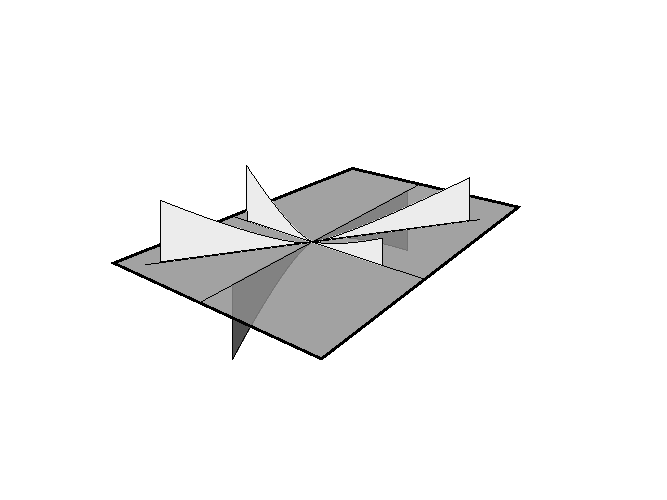
\includegraphics{figures/03secondderivatives.pdf}
    \caption{ Second derivative in several directions}
    \label{fig:03second-derivatives}
\end{figure}

\section{Problems with constraints} Lagrange multipliers with one  %{{{2
constraint.  If the function $z=f(x, y)$ attains its largest value among
all points which satisfy the constraint $g(x, y) = C$ at the point $(a,
b)$, and if
\begin{equation}
  \nab g(a,b) \neq 0 ,
\end{equation}
then the point $(a, b)$ satisfies the \textit{Lagrange Multiplier}
equations,
\begin{equation}
  \nab f(a, b) = \lambda \nab g(a, b)
  \label{eq:Lagrange-multiplier} 
\end{equation}


\section{Problems}\small\sffamily %{{{2


\problem\label{pblm:find-critical-points}
Find all critical points of the following functions.  
Classify them into local/global maxima/minima, saddles, or other kind
of ciritical points.

\begin{tabbing}
\quad\=\subprob $f(x,y)=x^2+4y^2-2x+8y-1$\qquad
\answer minimum at $(1,-1)$
\endanswer
\=\subprob $f(x,y)=x^2-y^2+6x-10y+2$
\answer none
\endanswer
\\
\>\subprob $f(x,y)=x^2+4xy+y^2-6y+1$
\answer none
\endanswer
\>
\subprob  $f(x,y)=x^2-xy+2y^2-5x+6y-9$
\answer  minimum at $(2,-1)$
\endanswer
\\
\>\subprob $f(x,y) = y^2-18 x^2+x^4$
\answer 
Global minima at $(\pm 3,0)$ and a saddle at the origin.
\endanswer
\>\subprob $f(x,y) = y^4-4y^2-18 x^2+x^4$
\answer  
There are nine critical points. Four global minima at $(\pm 3,
\pm\sqrt{3})$, four saddle points at $(0,\pm\sqrt{3})$ and $(\pm3,0)$
respectively, and finally, a local but not global maximum at the
origin.
\endanswer
\\
\>\subprob $f(x,y)=9+4x-y-2x^2-3y^2$
\answer maximum at $(1,-1/6)$
\endanswer
\>
\subprob $f(x,y)=xy(4-x-2y)$
\answer 
\endanswer
\\
\>\subprob $f(x,y)=(x-y^2)(x-1)$
\answer  
\endanswer
\>
\subprob $f(x,y)=(x-y)(xy-4)$
\answer  $(2,2)$ and $(-2,-2)$
\endanswer
\\
\>\subprob $f(x,y)=y^2+\cos x$
\answer  
\endanswer
\>
\subprob $f(x,y)=x^2y-\frac13 y^3$
\answer The origin. Neither a local max, min, nor saddle.
The graph of this function is called the ``Monkey Saddle'' as
it accomodates two legs and a tail too.
\endanswer
\\
\>\subprob $f(x,y)=(x-y^2)(x-1)$
\answer  
\endanswer
\>
\subprob $f(x,y)=(x-y)(xy-4)$
\answer  $(2,2)$ and $(-2,-2)$
\endanswer
\\
\>\subprob $f(x,y) = x^2$
\answer  All points on the $y$-axis are critical points.  They are all
global maxima, but the second derivative test doesn't tell you so.
\endanswer
\>\subprob $f(x,y) = x^2y$
\answer
All points on the $y$-axis are again critical points.  Those with
$y>0$ are local minima, those with $y<0$ are local maxima, and the
origin is neither.  The second derivative test applies to none of
these points.
\endanswer
\\
\>\subprob $f(x,y) = \bigl(1-x^2-y^2\bigr)^2$
\answer  All points on the unit circle are global minima, because the
function vanishes there, and is positive everywhere else.  The origin
is a local maximum.  The 2nd derivative test applies to the origin,
but not to any of the other critical points.
\endanswer
\>\subprob $f(x,y) = x^2y$
\answer
All points on the $y$-axis are again critical points.  Those with
$y>0$ are local minima, those with $y<0$ are local maxima, and the
origin is neither.  The second derivative test applies to none of
these points.
\endanswer
\end{tabbing}



\problem A six-sided rectangular box is to hold $1/2$ cubic meter.  Which
shape should the box be to minimize surface area?
\answer
Let the sides of the box be $x,y,z$.  We want to minimize the quantity $A =
2xy+2yz+2xz$, with the constraint $V=xyz=1/2$.  The constraint implies that
$x\neq$, $y\neq0$ and $z\neq0$ moreover, given $x$ and $y$ the only $z$
which satisfies the constraint is $z=1/(2xy)$.  Thus we must minimize the
following function of two variables
\[
A(x,y) = xy + \frac{1} {2x} + \frac{1} {2y}
\]
over all $x>0$, $y>0$.

A minimum must be an interior minimum (can't be on the $x$ or $y$-axis
since these are excluded), and thus must be a critical point.
\[
\pdd Ax = y-\frac{1} {2x^2}, \qquad
\pdd Ay = x - \frac{1} {2y^2}.
\]
Solving $A_x=A_y=0$ for $(x,y)$ leads to $x=y=\sqrt[3]2$, so the solution
is a cube $1/\sqrt[3]{2}$ on a side
\endanswer

\problem The post office will accept packages whose combined length and
girth is at most 130 inches (girth is the maximum distance around the
package perpendicular to the length). What is the largest volume that can
be sent in a rectangular box? 
\answer  $65/3\times 65/3\times 130/3$
\endanswer

\problem The bottom of a rectangular box costs twice as much per unit area
as the sides and top. Find the shape for a given volume that will minimize
cost. 
\answer  It has a square base, and is one and one half times as tall
as wide.  If the volume is $V$ the dimensions are $\root 3 \of {2V/3}\times
\root 3 \of {2V/3}\times \root 3\of {9V/4}$.
\endanswer

\problem Using the methods of this section, find the shortest distance from
the origin to the plane $x+y+z=10$. 
\answer  $\sqrt{100/3}$
\endanswer

\problem Using the methods of this section, find the shortest distance from
the point $(x_0,y_0,z_0)$ to the plane $ax+by+cz=d$.  You may assume that
$c\not=0$; use of Maple or similar software is recommended. 
\answer 
$|ax_0+by_0+cz_0-d|/\sqrt{a^2+b^2+c^2}$
\endanswer

\problem A trough is to be formed by bending up two sides of a long metal
rectangle so that the cross-section of the trough is an isosceles
trapezoid, as in figure~\ref{fig:trough}. If the width of the metal sheet
is 2 meters, how should it be bent to maximize the volume of the trough?
\answer The sides and bottom should all be $2/3$ meter, and the sides
should be bent up at angle $\pi/3$.
\endanswer

\problem Given the three points $(1,4)$, $(5,2)$, and $(3,-2)$,
$\DS(x-1)^2+(y-4)^2+(x-5)^2+(y-2)^2+(x-3)^2+(y+2)^2$ is the sum of the
squares of the distances from point $(x,y)$ to the three points. Find $x$
and $y$ so that this quantity is minimized. 
\answer  $(3,4/3)$
\endanswer

\problem Suppose that $f(x,y)=x^2+y^2+kxy$. Find and classify the critical
points, and discuss how they change when $k$ takes on different values.

\problem Find the shortest distance from the point $(0,b)$ to the parabola
$y=x^2$.

\problem Find the shortest distance from the point $(0,0,b)$ to the
paraboloid $z=x^2+y^2$.

\problem Consider the function $f(x,y)=x^3-3x^2y$.

\subprob Show that $(0,0)$ is the only critical point of $f$.

\subprob Show that the discriminant test is inconclusive for $f$.

\subprob Determine the traces of $f$ obtained by setting $x=k$ for various
values of $k$.

\subprob What kind of critical point is $(0,0)$?


\problem Find the volume of the largest rectangular box with edges parallel
to the axes that can be inscribed in the ellipsoid $2x^2+72y^2+18z^2=288$.





\problem A six-sided rectangular box is to hold $1/2$ cubic meter; what
shape should the box be to minimize surface area? 
\answer  a cube
\endanswer

\problem The post office will accept packages whose combined length and
girth are at most 130 inches (girth is the maximum distance around the
package perpendicular to the length). What is the largest volume that can
be sent in a rectangular box? 
\answer  $65/3\times 65/3\times 130/3$
\endanswer

\problem The bottom of a rectangular box costs twice as much per unit area
as the sides and top. Find the shape for a given volume that will minimize
cost. 
\answer  It has a square base, and is one and one half times as tall
as wide.  If the volume is $V$ the dimensions are $\root 3 \of {2V/3}\times
\root 3 \of {2V/3}\times \root 3\of {9V/4}$.
\endanswer

\problem Using Lagrange multipliers, find the shortest distance from the
point $(x_0,y_0,z_0)$ to the plane $ax+by+cz=d$. 
\answer 
$|ax_0+by_0+cz_0-d|/\sqrt{a^2+b^2+c^2}$
\endanswer

\problem Find all points on the surface $xy-z^2+1=0$ that are closest to
the origin. 
\answer  $(0,0,1)$, $(0,0,-1)$
\endanswer

\problem The material for the bottom of an aquarium costs half as much as
the high strength glass for the four sides. Find the shape of the cheapest
aquarium that hold a given volume $V$. 
\answer  $\root 3\of{4V}\times\root
3\of{4V}\times\root 3\of{V/16}$
\endanswer

\problem The plane $x-y+z=2$ intersects the cylinder $x^2+y^2=4$ in an
ellipse. Find the points on the ellipse closest to and farthest from the
origin. 
\answer  Farthest: $(-\sqrt2,\sqrt2,2+2\sqrt2)$; closest:
$(2,0,0)$, $(0,-2,0)$
\endanswer


%%% Local Variables: 
%%% mode: latex
%%% TeX-master: "free234"
%%% End: 

